\documentclass{curs}

% Comment out lines below in case of no code to be included.
%\usepackage{code/highlight}
\usepackage{color}
\usepackage{graphicx}
\usepackage{listings}
\usepackage{multicol}
%\usepackage{alltt}


\title[Session 08]{Session 08}
\subtitle{System Isolation}
\author{Security of Information Systems (SIS)}
\date{November 16, 2017}

\begin{document}

\frame{\titlepage}

\section{Confinement}

\begin{frame}{Run Untrusted Code}
  \begin{itemize}
    \item apps, plugins, codecs
    \item software not written by you, not-verified
    \item damage control
    \item kill it if it misbehaves
    \item ensure misbehaving app does not alter the system
  \end{itemize}
\end{frame}

\begin{frame}{Confinement Types}
  \begin{itemize}
    \item hardware: different hardware systems, air gap
    \item virtual machine: isolate OSes in a single machine
    \item process: sandboxing, jailing
    \item application: software fault isolation
  \end{itemize}
\end{frame}

\begin{frame}{Software Fault Isolation}
  \begin{itemize}
    \item isolate components in their \textit{fault domain}
    \item part of the same address space
    \item requires some OS/hardware support to separate addresses
    \item Mogoșanu et al.: MicroStache: A Lightweight Execution Context for In-Process Safe Region Isolation
  \end{itemize}
\end{frame}

\begin{frame}{Reference Monitor}
  \begin{itemize}
    \item mediates requests, implements policy, enforces isolation and confinement
    \item must always be invoked
    \item tamperproof
    \item validated
  \end{itemize}
\end{frame}

\section{System Isolation. Trusted Computing Base}

\begin{frame}{Principles and Goals}
  \begin{itemize}
    \item least privilege
    \item privilege separation
    \item safely execute a non-trusted program
    \item harden a system that runs programs that increase its attack surface
    \item isolate what can happen if a vulnerability is exploited
  \end{itemize}
\end{frame}

\begin{frame}{Mechanism and Policy}
  \begin{itemize}
    \item mechanism: how goals are achieved
    \item policy: rules that achieve isolation goals
    \item mechanism: mostly implementation
    \item policy: mostly configuration
  \end{itemize}
\end{frame}

\begin{frame}{Mechanisms and Policies}
  \begin{figure}
    \centering
    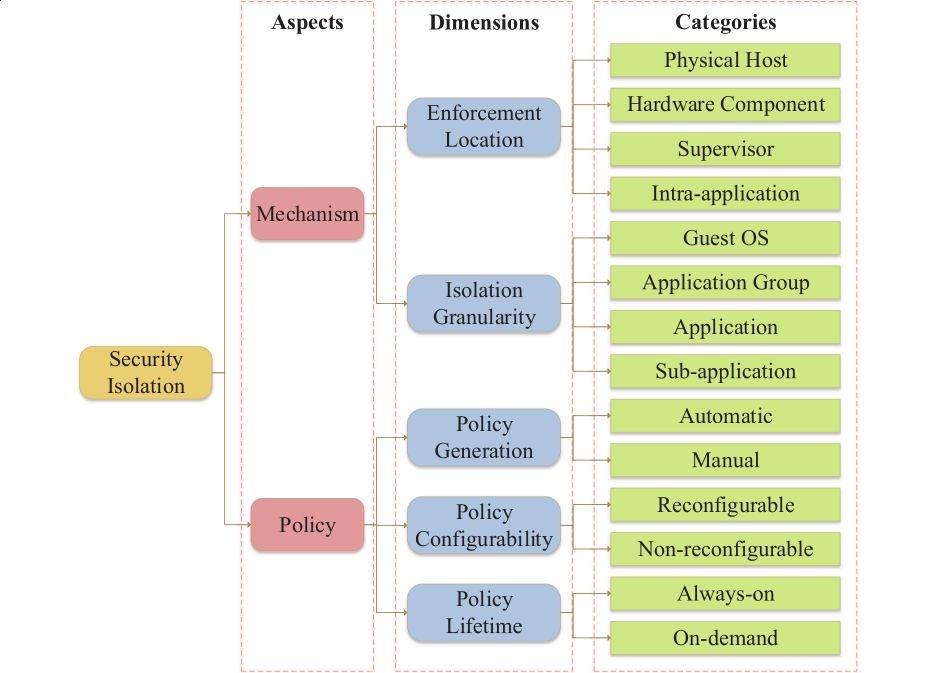
\includegraphics[width=\textwidth]{img/isolation-mechanism-policy} \\
    {\tiny Rui Shu et al.: A Study of Security Isolation Techniques}
  \end{figure}
\end{frame}

\begin{frame}{System Isolation}
  \begin{itemize}
    \item isolate app, group apps or entire OS
    \item prevent it from hurting other components
    \item virtual machines, library OS, containers
    \item we consider sandboxing, mandatory access control, software fault isolation (SFI) to be app-centric mechanisms (not system-centric)
  \end{itemize}
\end{frame}

\begin{frame}{Trusted Computing Base (TCB)}
  \begin{itemize}
    \item trusted system components (by the reference monitor)
    \item critical parts of the system
    \item if exploited, might jeopardize the security of the entire system
    \item aimed to be small (reduced attack surface)
  \end{itemize}
\end{frame}

\section{Hardware Components}

\begin{frame}{Hardware Protection}
  \begin{itemize}
    \item provide security isolation for shared resources
    \item passive components: TPM (\textit{Trusted Platform Module})
    \item active components: control critical system operations
  \end{itemize}
\end{frame}

\begin{frame}{Trusted Execution Environment (TEE)}
  \begin{itemize}
    \item secure are on CPU
    \item code run is secure: confidentiality and integrity
    \item runs in parallel with OS
  \end{itemize}
\end{frame}

\begin{frame}{Intel TXT}
  \begin{itemize}
    \item Trusted eXecution Technology
    \item attest platform/operating system
    \item uses TPM and cryptography to validate/measure code that can be trusted
  \end{itemize}
\end{frame}

\begin{frame}{ARM TrustZone}
  \begin{itemize}
    \item ARM TZ
    \item two worlds: secure and non-secure
    \item rich OS runs in non-secure worlds, security-specialized code in secure world
    \item aim to reduce attack surface
  \end{itemize}
\end{frame}

\begin{frame}{Intel SGX}
  \begin{itemize}
    \item Software Guard eXtensions
    \item specialized instructions
    \item user-level code allocates enclaves
    \item protected from higher privilege level components
    \item secure remote computation
    \item cache DRAM side-channel attack
  \end{itemize}
\end{frame}

\begin{frame}{Secure Enclave}
  \begin{itemize}
    \item on Apple iOS / watchOS devices
    \item fingerprint data completely walled from the OS
    \item uses a SEP (\textit{Secure Enclave Processor}), SEP OS
    \item based on ARM TZ
  \end{itemize}
\end{frame}

\section{Virtualization}

\begin{frame}{Virtualization}
  \begin{figure}
    \centering
    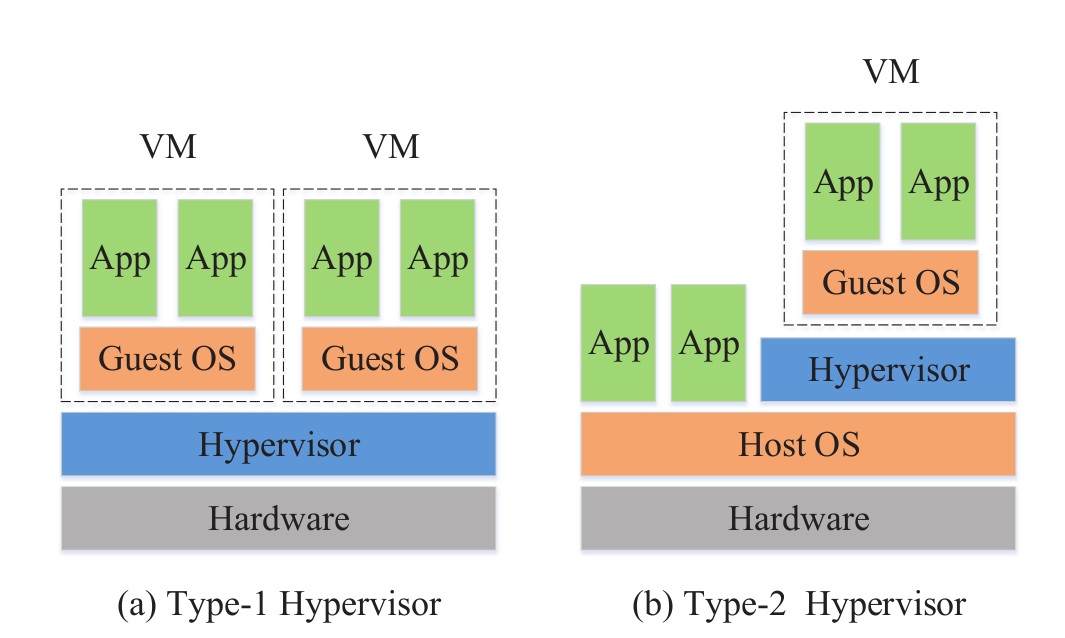
\includegraphics[width=0.9\textwidth]{img/virtualization} \\
    {\tiny Rui Shu et al.: A Study of Security Isolation Techniques}
  \end{figure}
\end{frame}

\begin{frame}{Virtual Machine}
  \begin{itemize}
    \item run an isolated OS instance on top of a supervisor component (hypervisor)
    \item hypervisor or VMM (\textit{Virtual Machine Monitor})
    \item malware in a VM cannot infect host OS or other VMs
  \end{itemize}
\end{frame}

\begin{frame}{Covert Channels}
  \begin{itemize}
    \item side channels
    \item use CPU, memory, cache information from one VM to determine what's happening on the other VM
  \end{itemize}
\end{frame}

\begin{frame}{VMM Detection}
  \begin{itemize}
    \item VM platforms emulate simple hardware
    \item VMM introduces time latency variances
    \item VMM shares TLB (\textit{Translation Lookaside Buffers})
  \end{itemize}
\end{frame}

\begin{frame}{Type-1 vs Type-2}
  \begin{itemize}
    \item reduced TCB vs additional flexibility
    \item efficiency for Type-1
  \end{itemize}
\end{frame}
\section{Library OS}

\begin{frame}{Library OS}
  \begin{figure}
    \centering
    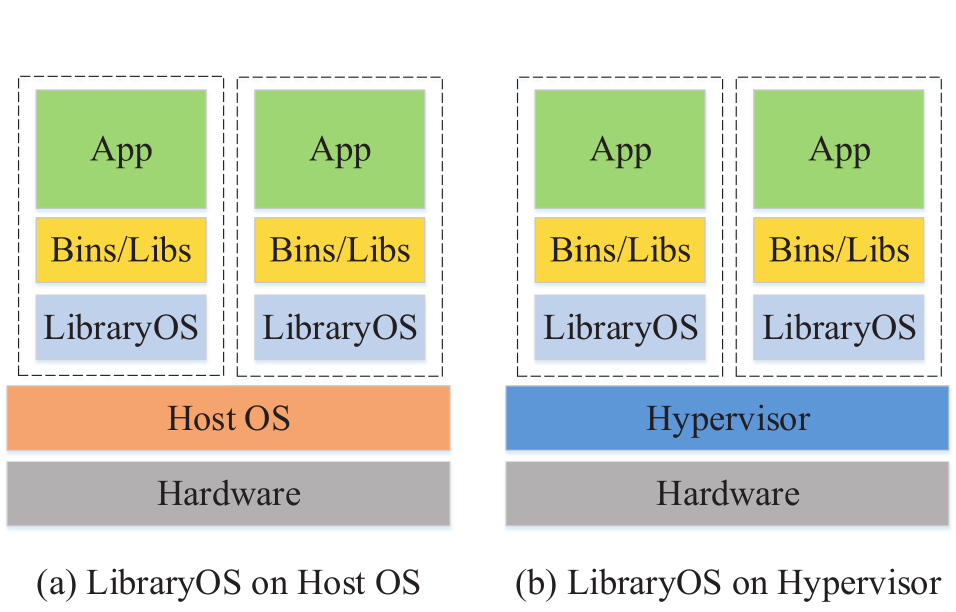
\includegraphics[width=0.9\textwidth]{img/library-os} \\
    {\tiny Rui Shu et al.: A Study of Security Isolation Techniques}
  \end{figure}
\end{frame}

\begin{frame}{Library OS Characteristics}
  \begin{itemize}
    \item unikernel
    \item OS functionality as user library/libraries
    \item single-image app, can run on top of hypervisor or hardware
    \item no need for user-level/kernel-level transitions
    \item difficult to run multiple instances: use a hypervisor
    \item reduce the attack surface
  \end{itemize}
\end{frame}

\begin{frame}{Implementations}
  \begin{itemize}
    \item ClickOS: virtualized software middle box
    \item LKL (\textit{Linux Kernel Library})
    \item My VM is Lighter (and Safer) than Your Container: \url{http://cnp.neclab.eu/projects/lightvm/lightvm.pdf}
  \end{itemize}
\end{frame}

\section{Containerization}

\begin{frame}{Containers}
  \begin{figure}
    \centering
    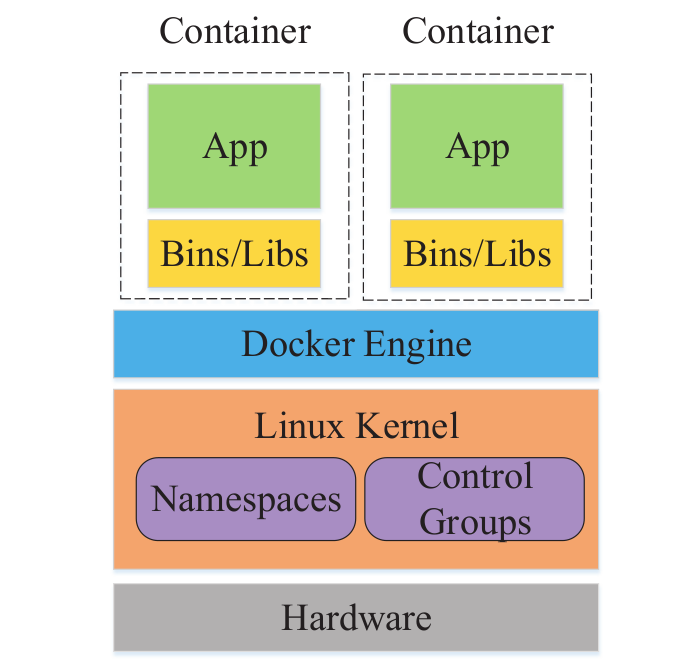
\includegraphics[width=0.7\textwidth]{img/container} \\
    {\tiny Rui Shu et al.: A Study of Security Isolation Techniques}
  \end{figure}
\end{frame}

\begin{frame}{Container}
  \begin{itemize}
    \item restricted environment
    \item applications or application groups
    \item sandboxing only provides a certain set of privileges
    \item containers provide a dedicated isolated environment
  \end{itemize}
\end{frame}

\begin{frame}{LXC/Docker}
  \begin{itemize}
    \item Linux Containers
    \item use Linux namespaces: PID, network, IPC, mount, user, UTS
    \item Linux control groups (cgroups): limits, accounts, isolates resource usage
  \end{itemize}
\end{frame}

\begin{frame}{OS vs. Application Containers}
  \begin{itemize}
    \item OS: provided an entire distro, similar to a virtual machine (LXC)
    \item app: provide an environment for running a single service (Docker)
  \end{itemize}
\end{frame}

\begin{frame}{Containers vs. hypervisors}
  \begin{itemize}
    \item containers are faster to create, deploy, run
    \item containers are lighter (reduced overhead)
    \item hypervisors are more secure: reduced TCB, no common kernel
  \end{itemize}
\end{frame}

\section{Summary}

\begin{frame}{Keywords}
  \begin{columns}
    \begin{column}{0.5\textwidth}
      \begin{itemize}
        \item confinement
        \item isolation
        \item resource monitor
        \item TCB
        \item TEE
        \item Intel TXT
        \item Intel SGX
      \end{itemize}
    \end{column}
    \begin{column}{0.5\textwidth}
      \begin{itemize}
        \item ARM TZ
        \item VMM
        \item hypervisor
        \item library OS
        \item unikernel
        \item container
        \item LXC
        \item Docker
      \end{itemize}
    \end{column}
  \end{columns}
\end{frame}

\begin{frame}{Resources}
  \begin{itemize}
    \item \href{https://dl.acm.org/citation.cfm?id=2988545}{A Study of Security Isolation Techniques}
    \item \href{https://crypto.stanford.edu/cs155/lectures/03-isolation.pdf}{CS155: Computer Security: Isolation}
    \item \url{https://blog.risingstack.com/operating-system-containers-vs-application-containers/}
  \end{itemize}
\end{frame}

\end{document}
